\documentclass[12pt,addpoints,answers]{repaso}
\grado{2}
\nivel{Secundaria}
\cicloescolar{2023-2024}
\materia{Matemáticas}
\unidad{3}
\title{Practica la Unidad}
\aprendizajes{
    \item Usa e interpreta las medidas de tendencia central (moda, media aritmética y mediana), y decide cuál de ellas conviene más en el análisis de los datos en cuestión.
    \item Resuelve problemas de proporcionalidad directa e inversa y de reparto proporcional.
    \item Verifica algebraicamente la equivalencia de expresiones de primer grado, formuladas a partir de sucesiones.    
    \item Resuelve problemas mediante la formulación y solución algebraica de ecuaciones lineales.  
}
\author{Melchor Pinto, J.C.}
\begin{document}
\INFO%
\section*   {Probabilidad y estadística}
% \subsection*{Mediana y moda}
\ejemplosboxed[{Contesta las siguientes preguntas:

            \begin{multicols}{2}
                \begin{parts}
                    \part Las calificaciones de un salón de secundaria son las siguientes: 80, 82, 85, 88, 90, 88, 91, 85, 95, 88, 88, 97, 100. ¿Cuál es la mediana de las calificaciones?
                    \fillin[88][2cm]

                    \begin{solutionbox}{2cm}
                        Ordenando los datos se obtiene:\\[-0.2em]
                        $\left\{80, 82, 85, 85, 88, 88, 88, 88, 90, 91, 95, 97, 100 \right\} $\\[-0.2em]
                        $\therefore$ Mediana es 88
                    \end{solutionbox}

                    \part Las edades de un grupo de personas son: 44, 41, 47, 48, 44, 39, 45, 49, 44 y 47 años. ¿Cuál es la mediana de las edades?
                    \fillin[44.5][2cm]

                    \begin{solutionbox}{2cm}
                        Ordenando los datos se obtiene: \\[-0.2em]
                        $\left\{39, 41, 44, 44, 44, 45, 47, 47, 48, 49 \right\} $ \\[-0.2em]
                        $\therefore$ Mediana es 44.5
                    \end{solutionbox}

                \end{parts}
            \end{multicols}
        }]

\begin{questions}
    \questionboxed[4]{Contesta las siguientes preguntas:

        \begin{multicols}{2}
            \begin{parts}
                \part Las calificaciones de un salón de secundaria son las siguientes: 5, 7, 6, 8, 7, 9, 10, 7, 8, 7, 9, 7. ¿Cuál es la mediana de las calificaciones?
                \fillin[7][2cm]

                \begin{solutionbox}{1.8cm}
                \end{solutionbox}

                \part Las edades de un grupo de personas son: 15, 17, 15, 18, 19, 14, 15, 13 y 17 años. ¿Cuál es la mediana de las edades?
                \fillin[15][2cm]

                \begin{solutionbox}{1.8cm}
                \end{solutionbox}

            \end{parts}
        \end{multicols}
    }
    % \subsection*{Promedio}

    \ejemplosboxed[{Contesta las siguientes preguntas:

                \begin{multicols}{2}
                    \begin{parts}
                        \part El número de goles en las últimas 3 temporadas de un delantero fueron: 22, 26 y 31, ¿cuál es el promedio de goles por temporada?
                        \fillin[26.33][2cm]

                        \begin{solutionbox}{2.5cm}
                            Para encontrar el promedio sumamos el total de goles en esas temporadas y luego dividimos esa suma por el número de temporadas. En este caso, el promedio es
                            $(22+26+31)/3=26.33$
                        \end{solutionbox}

                        \part En un grupo de 11 personas se registraron los siguientes pesos: 62, 64, 65, 59, 68, 72, 77, 71, 82, 69 y 76 kg. ¿Cuál es el promedio de los pesos?
                        \fillin[69.54][2cm]

                        \begin{solutionbox}{2.5cm}
                            Al sumar los pesos: 62 + 64 + 65 + 59 + 68 + 72 + 77 + 71 + 82 + 69 + 76 = 765 kg, y dividir por 11 personas, obtenemos un promedio de aproximadamente 69.55 kg.
                        \end{solutionbox}

                    \end{parts}
                \end{multicols}
            }]

    \questionboxed[4]{Contesta las siguientes preguntas:

        \begin{multicols}{2}
            \begin{parts}
                \part Las estaturas de un grupo de personas son: 171, 172, 168, 166, 164, 178 y 175 cm, ¿cuál es el promedio de la estatura de las personas?
                \fillin[170.57][2cm]

                \begin{solutionbox}{2cm}

                \end{solutionbox}

                \part En un grupo de 9 personas se registraron los siguientes pesos: 87, 60, 71, 74, 81, 80, 66, 74 y 79 kg. ¿Cuál es el promedio de los pesos?
                \fillin[74.66][2cm]

                \begin{solutionbox}{2cm}
                \end{solutionbox}

            \end{parts}
        \end{multicols}
    }

    % \subsection*{Interpretación de gráficas}
    \ejemplosboxed[{Los resultados de una encuesta se muestran en la siguiente gráfica de barras:

                \begin{multicols}{2}
                    \begin{parts}
                        \part  ¿Cuántas personas participaron en la encuesta? \fillin[95][2cm]
                        \part  ¿Cuál es la fruta menos preferida por las personas? \fillin[Naranja][2cm]
                        \part  ¿Cuál es la fruta preferida por las personas? \fillin[Manzana][2cm]

                        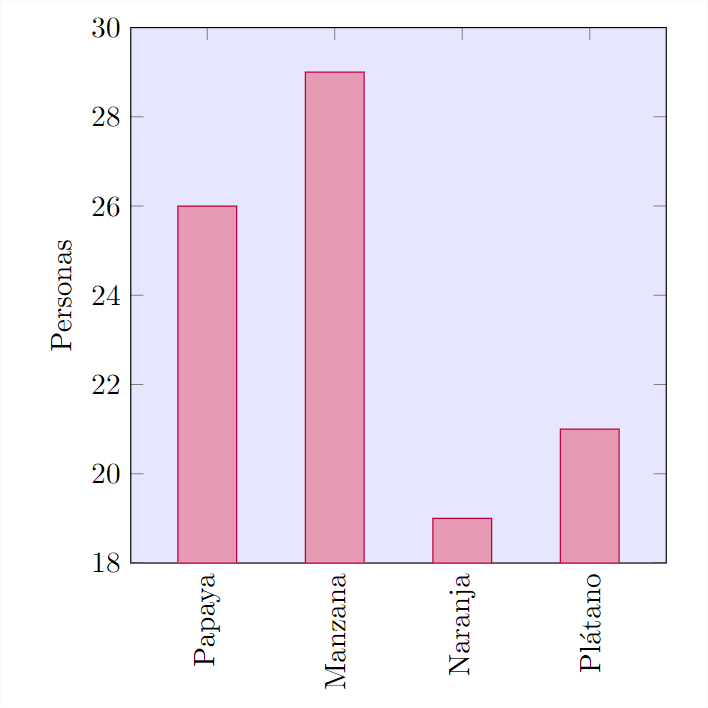
\includegraphics[width=.85\linewidth]{mexmat00001.png}
                    \end{parts}
                \end{multicols}
            }]

    \questionboxed[3]{Los resultados de una encuesta se muestran en la siguiente gráfica de barras:

        \begin{multicols}{2}
            \begin{parts}
                \part  ¿Cuántas personas participaron en la encuesta? \fillin[70][2cm]
                \part  ¿Cuál es la fruta menos preferida por las personas? \fillin[Papaya][2cm]
                \part  ¿Cuál es la fruta preferida por las personas? \fillin[Plátano][2cm]

                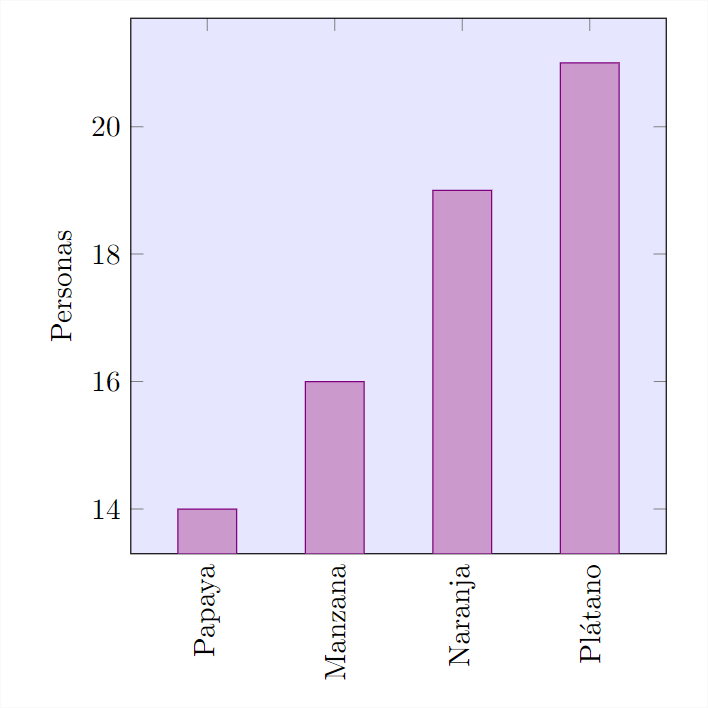
\includegraphics[width=.85\linewidth]{mexmat00001a.png}
            \end{parts}
        \end{multicols}
    }

    % \subsection*{Eventos mutuamente excluyentes}

    \questionboxed[3]{Resuelve los siguientes problemas:

        \begin{multicols}{3}

            \begin{parts}
                \part En una urna hay 10 pelotas azules, 5 verdes, 15 blancas y 20 negras. Calcula la probabilidad de sacar una pelota negra.

                \begin{solutionbox}{3cm}
                \end{solutionbox}

                \columnbreak%

                \part Si se lanzan tres monedas al aire, calcula la probabilidad de que caiga puro sol.

                \begin{solutionbox}{3cm}
                \end{solutionbox}

                \columnbreak%

                \part En una urna hay 8 pelotas moradas, 12 naranjas, 7 rojas, 11 azules y 7 blancas. Calcula la probabilidad de sacar una pelota negra.

                \begin{solutionbox}{3cm}
                \end{solutionbox}
            \end{parts}
        \end{multicols}
    }

    % \subsection*{Eventos dependientes e independientes}

    \questionboxed[3]{Resuelve los siguientes problemas:
        \begin{multicols}{2}

            \begin{parts}
                \part Se lanza una moneda al aire y al mismo tiempo un dado, ¿cuál es la probabilidad de que caiga águila en la moneda y el número 2 en el dado?
                \fillin[1/12][2cm]

                \begin{solutionbox}{2cm}
                \end{solutionbox}

                \part Al lanzar un dado tres veces consecutivas, ¿qué probabilidad hay de obtener en el primer dado un 2, en el segundo un 3 y en el tercero un número impar?
                \fillin[1/72][2cm]

                \begin{solutionbox}{2cm}
                \end{solutionbox}

            \end{parts}
        \end{multicols}
    }

    \section*   {Razones y proporciones}
    % \subsection*{Relaciones proporcionales}

    \ejemplosboxed[{Determina si las siguientes tablas de datos son o no una relación proporcional:

                \begin{multicols}{2}
                    \begin{parts}
                        \part
                        \begin{minipage}[t]{0.4\linewidth}
                            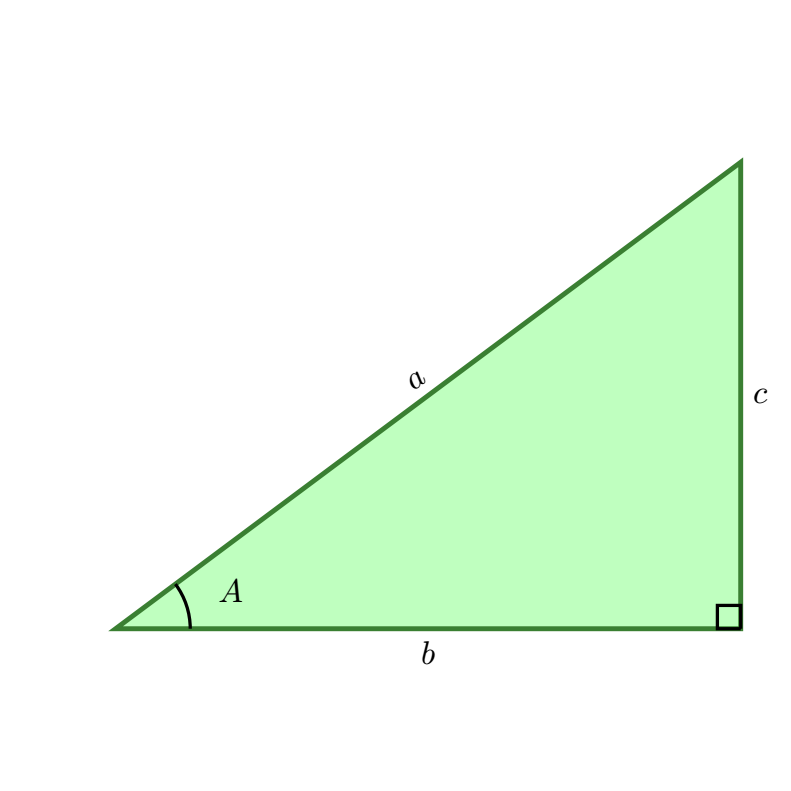
\includegraphics[width=\textwidth]{mex_0071.png}
                        \end{minipage}%
                        \begin{minipage}[b]{0.6\linewidth}
                            \begin{choices}
                                \choice Propocional
                                \CorrectChoice No proporcional
                            \end{choices}
                        \end{minipage}

                        \begin{solutionbox}{3cm}
                            $7\div 1=7$\\[-0.2em]
                            $9\div 2=4.5$\\[-0.2em]
                            $11\div 3=3.\overline{6}$\\[-0.2em]
                            $13\div 4=3.25$\\[-0.2em]
                            $15\div 5=3$\\[-0.2em]
                            $\therefore$ es una relación no proporcional.
                        \end{solutionbox}


                        % \part 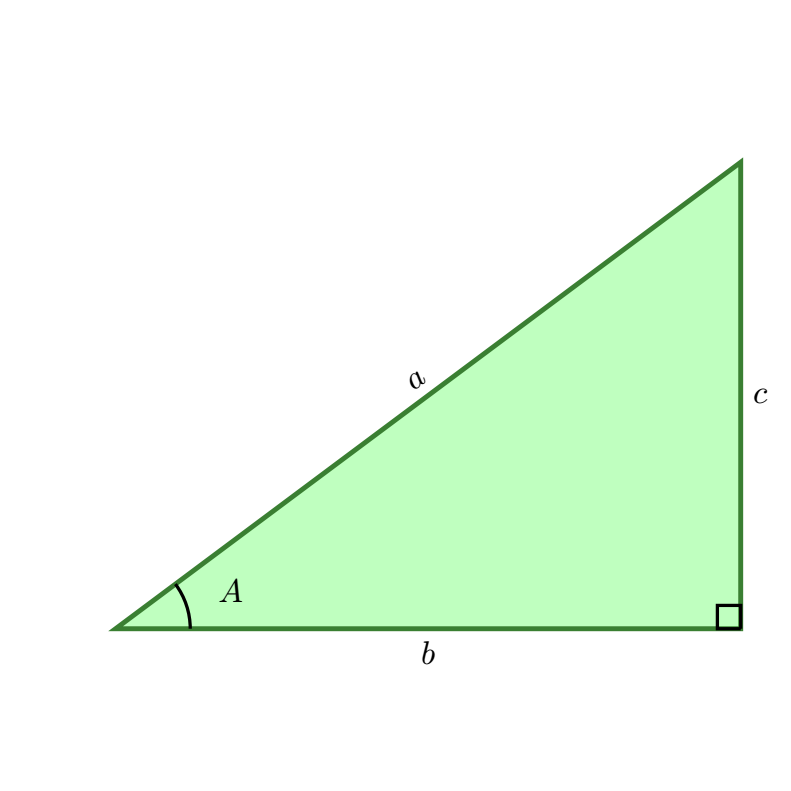
\includegraphics[width=.7\linewidth]{mex_0071.png}

                        % \begin{choices}
                        %     \choice Propocional
                        %     \choice No proporcional
                        % \end{choices}

                        \part
                        \begin{minipage}[t]{0.4\linewidth}
                            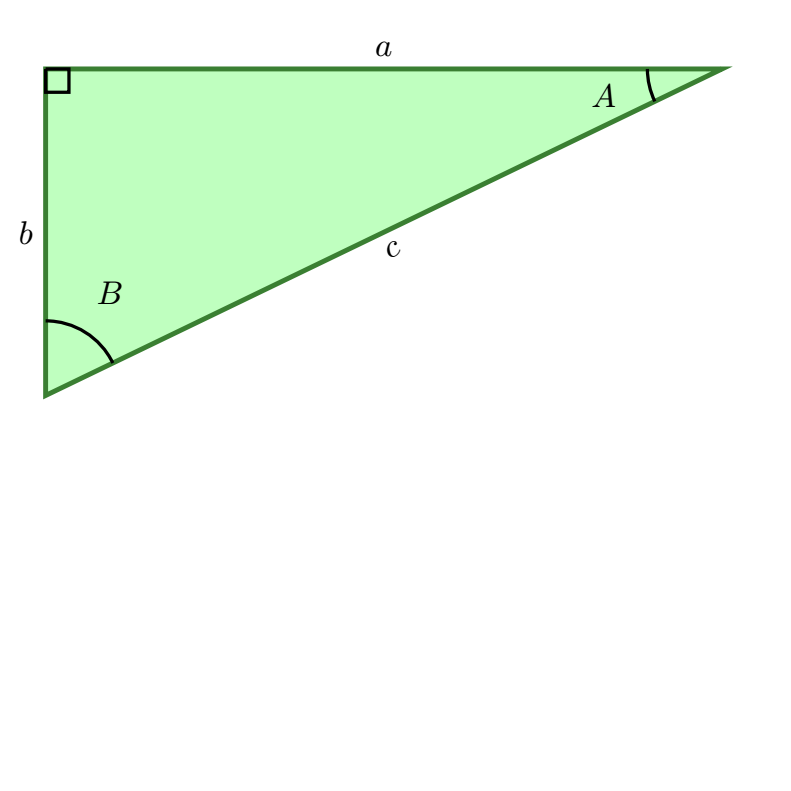
\includegraphics[width=\textwidth]{mex_0072.png}
                        \end{minipage}%
                        \begin{minipage}[b]{0.6\linewidth}
                            \begin{choices}
                                \CorrectChoice Propocional
                                \choice No proporcional
                            \end{choices}
                        \end{minipage}

                        \begin{solutionbox}{3cm}
                            $43.2\div 18=2.4$\\[-0.2em]
                            $33.6\div 14=2.4$\\[-0.2em]
                            $24\div 10=2.4$\\[-0.2em]
                            $14.4\div 6=2.4$\\[-0.2em]
                            $4.8\div 2=2.4$\\[-0.2em]
                            $\therefore$ es una relación proporcional.
                        \end{solutionbox}


                    \end{parts}
                \end{multicols}
            }]

    \questionboxed[6]{Determina si las siguientes tablas de datos son o no una relación proporcional:

        \begin{multicols}{2}
            \begin{parts}
                \part
                \begin{minipage}[t]{0.35\linewidth}
                    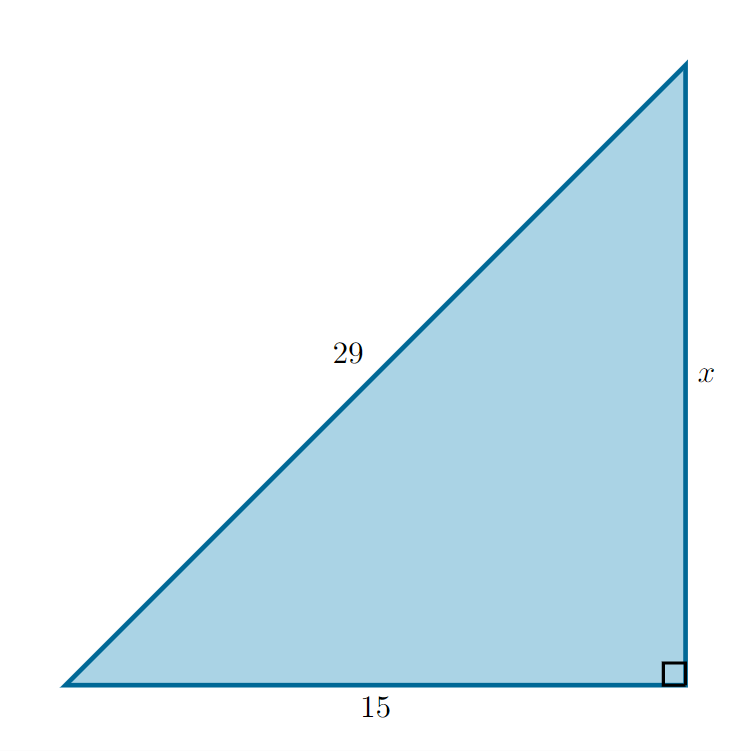
\includegraphics[width=\textwidth]{mex_0064.png}
                \end{minipage}%
                \begin{minipage}[b]{0.6\linewidth}
                    \begin{choices}
                        \choice Propocional
                        \CorrectChoice No proporcional
                    \end{choices}
                \end{minipage}

                \begin{solutionbox}{2.3cm}\small%

                    \begin{multicols}{3}
                        $7\div 1=7$\\[-0.2em]
                        $9\div 2=4.5$\\[-0.2em]

                        \columnbreak% 

                        $11\div 3=3.\overline{6}$\\[-0.2em]
                        $13\div 4=3.25$\\[-0.2em]
                        $15\div 5=3$

                        \columnbreak% 

                        $\therefore$ relación no proporcional.
                    \end{multicols}

                \end{solutionbox}

                \part
                \begin{minipage}[t]{0.35\linewidth}
                    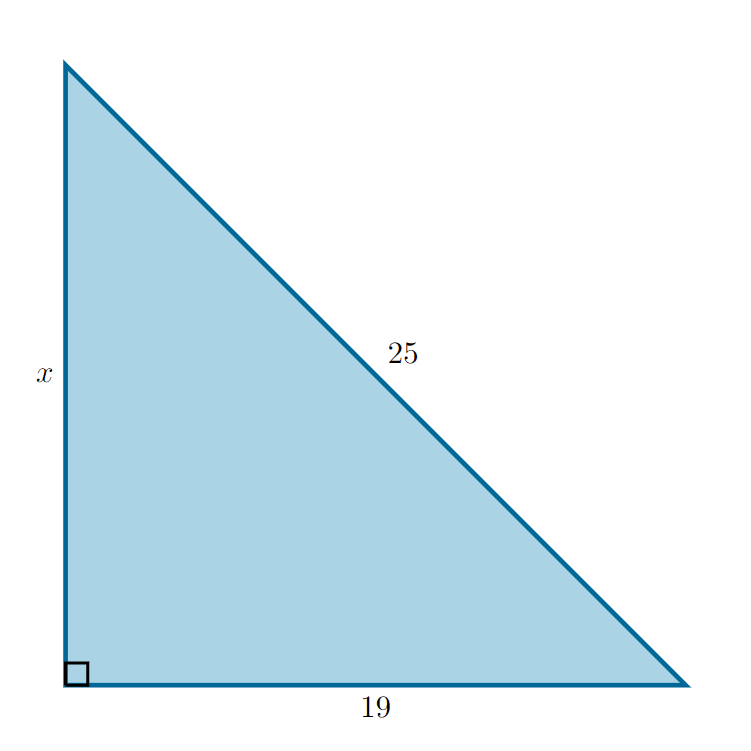
\includegraphics[width=\textwidth]{mex_0065.png}
                \end{minipage}%
                \begin{minipage}[b]{0.6\linewidth}
                    \begin{choices}
                        \choice Propocional
                        \CorrectChoice No proporcional
                    \end{choices}
                \end{minipage}

                \begin{solutionbox}{2.3cm}\small%

                    \begin{multicols}{3}
                        $7\div 1=7$\\[-0.2em]
                        $9\div 2=4.5$\\[-0.2em]

                        \columnbreak% 

                        $11\div 3=3.\overline{6}$\\[-0.2em]
                        $13\div 4=3.25$\\[-0.2em]
                        $15\div 5=3$

                        \columnbreak% 

                        $\therefore$ relación no proporcional.
                    \end{multicols}

                \end{solutionbox}

                \part
                \begin{minipage}[t]{0.35\linewidth}
                    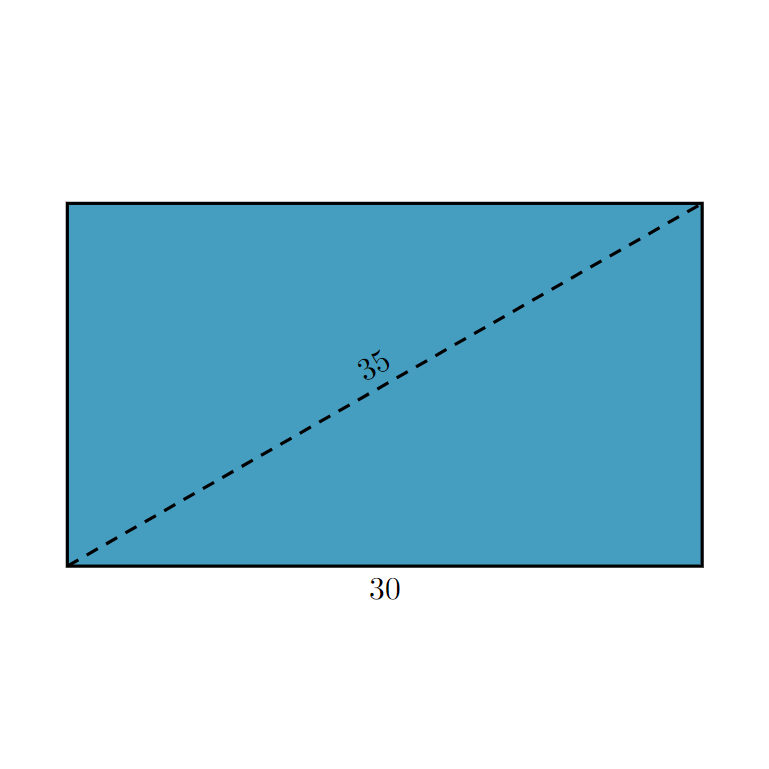
\includegraphics[width=\textwidth]{mex_0066.png}
                \end{minipage}%
                \begin{minipage}[b]{0.6\linewidth}
                    \begin{choices}
                        \choice Propocional
                        \CorrectChoice No proporcional
                    \end{choices}
                \end{minipage}

                \begin{solutionbox}{2.3cm}\small%

                    \begin{multicols}{3}
                        $7\div 1=7$\\[-0.2em]
                        $9\div 2=4.5$\\[-0.2em]

                        \columnbreak% 

                        $11\div 3=3.\overline{6}$\\[-0.2em]
                        $13\div 4=3.25$\\[-0.2em]
                        $15\div 5=3$

                        \columnbreak% 

                        $\therefore$ relación no proporcional.
                    \end{multicols}

                \end{solutionbox}

                \part
                \begin{minipage}[t]{0.35\linewidth}
                    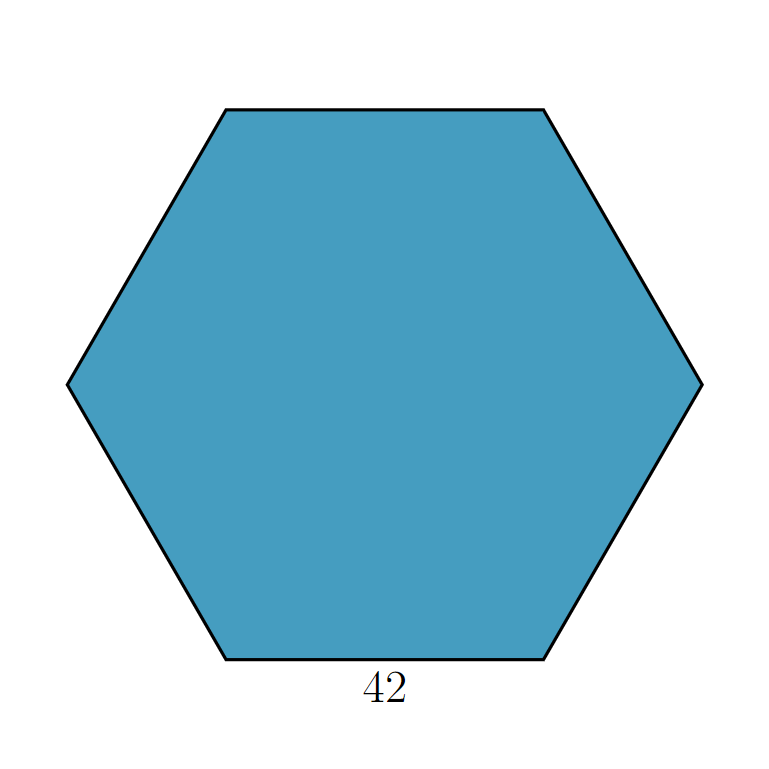
\includegraphics[width=\textwidth]{mex_0067.png}
                \end{minipage}%
                \begin{minipage}[b]{0.6\linewidth}
                    \begin{choices}
                        \choice Propocional
                        \CorrectChoice No proporcional
                    \end{choices}
                \end{minipage}

                \begin{solutionbox}{2.5cm}\small%

                    \begin{multicols}{3}
                        $7\div 1=7$\\[-0.2em]
                        $9\div 2=4.5$\\[-0.2em]

                        \columnbreak% 

                        $11\div 3=3.\overline{6}$\\[-0.2em]
                        $13\div 4=3.25$\\[-0.2em]
                        $15\div 5=3$

                        \columnbreak% 

                        $\therefore$ relación no proporcional.
                    \end{multicols}
                \end{solutionbox}

                % \part
                % \begin{minipage}[t]{0.4\linewidth}
                %     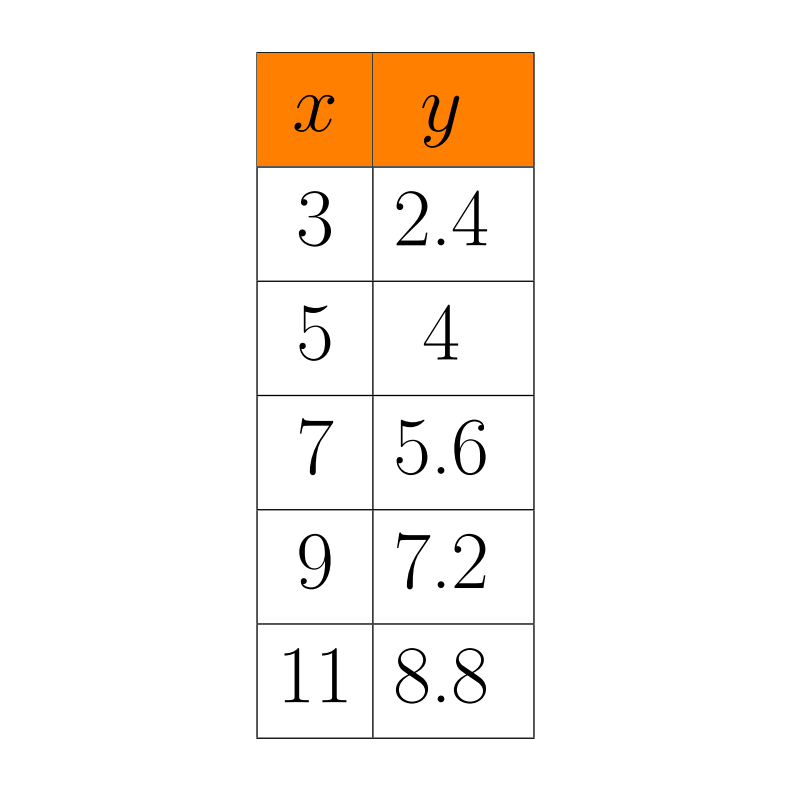
\includegraphics[width=\textwidth]{mex_0068.png}
                % \end{minipage}%
                % \begin{minipage}[b]{0.6\linewidth}
                %     \begin{choices}
                %         \choice Propocional
                %         \CorrectChoice No proporcional
                %     \end{choices}
                % \end{minipage}

                % \begin{solutionbox}{3cm}\small%
                %     $7\div 1=7$\\[-0.2em]
                %     $9\div 2=4.5$\\[-0.2em]
                %     $11\div 3=3.\overline{6}$\\[-0.2em]
                %     $13\div 4=3.25$\\[-0.2em]
                %     $15\div 5=3$\\[-0.2em]
                %     $\therefore$ es una relación no proporcional.
                % \end{solutionbox}

                % \part
                % \begin{minipage}[t]{0.4\linewidth}
                %     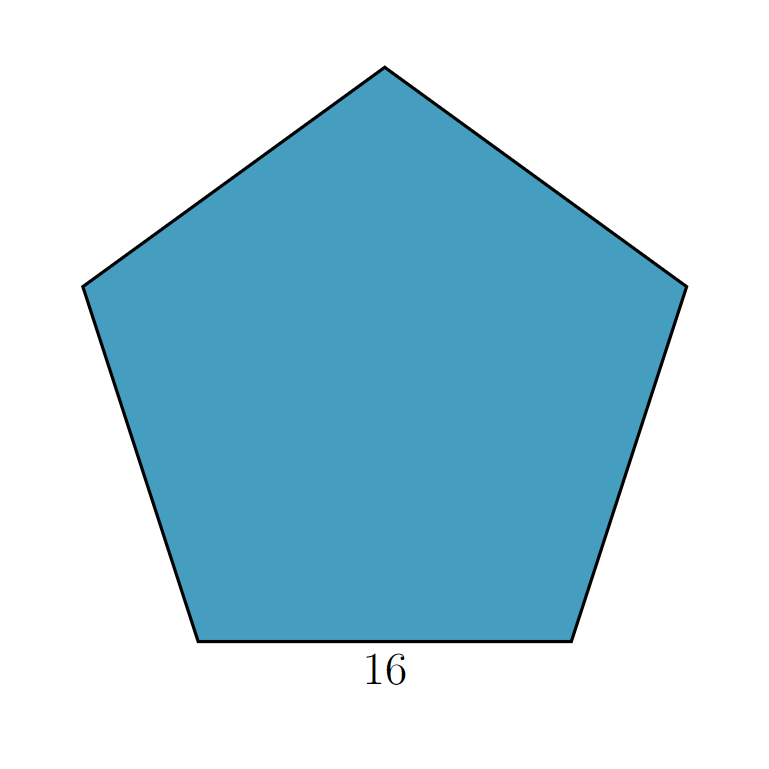
\includegraphics[width=\textwidth]{mex_0069.png}
                % \end{minipage}%
                % \begin{minipage}[b]{0.6\linewidth}
                %     \begin{choices}
                %         \choice Propocional
                %         \CorrectChoice No proporcional
                %     \end{choices}
                % \end{minipage}

                % \begin{solutionbox}{3cm}\small%
                %     $7\div 1=7$\\[-0.2em]
                %     $9\div 2=4.5$\\[-0.2em]
                %     $11\div 3=3.\overline{6}$\\[-0.2em]
                %     $13\div 4=3.25$\\[-0.2em]
                %     $15\div 5=3$\\[-0.2em]
                %     $\therefore$ es una relación no proporcional.
                % \end{solutionbox}
            \end{parts}
        \end{multicols}
    }

    % \subsection*{Constante de proporcionalidad}


    % \subsection*{Regla de correspondencia}


    % \subsection*{Proporción directa e inversa}


    % \subsection*{Proporciones compuestas}


    \section*   {Sucesiones aritméticas}
    % \subsection*{Completando la sucesión}


    % \subsection*{Diferencia de una sucesión}


    % \subsection*{Término enésimo}
    % \subsection*{Término general}
    % \subsection*{Término enésimo 2}



    \section*   {Ecuaciones lineales}
    % \subsection*{Lenguaje algebraico}


    % \subsection*{Sustitución de valores}


    % \subsection*{Ecuaciones de primer grado 1}
    % \subsection*{Ecuaciones de primer grado 2}


    % \subsection*{Resolución de problemas}


    \section*   {Sistemas de ecuaciones}
    % \subsection*{Método de eliminación}


    % \subsection*{Método de sustitución}


    % \subsection*{Método de igualación}


    % \subsection*{Sistema de ecuaciones 2x2 1}


    % \subsection*{Sistema de ecuaciones 2x2}


\end{questions}
\end{document}